% Created 2022-06-21 Tue 15:13
% Intended LaTeX compiler: pdflatex
\documentclass[11pt]{article}
\usepackage[utf8]{inputenc}
\usepackage[T1]{fontenc}
\usepackage{graphicx}
\usepackage{longtable}
\usepackage{wrapfig}
\usepackage{rotating}
\usepackage[normalem]{ulem}
\usepackage{amsmath}
\usepackage{amssymb}
\usepackage{capt-of}
\usepackage{hyperref}
\hypersetup{colorlinks=true,linkcolor=grey}
\author{Youssef}
\date{\today}
\title{}
\hypersetup{
 pdfauthor={Youssef},
 pdftitle={},
 pdfkeywords={},
 pdfsubject={},
 pdfcreator={Emacs 28.1 (Org mode 9.5.4)}, 
 pdflang={English}}
\begin{document}

\tableofcontents

\setlength{\parindent}{0pt}
\section{Dispensation En Pédiatrie}
\label{sec:orgcbc7d22}
\subsection{Classes d'âge}
\label{sec:org9eb9cdc}
\begin{center}
\begin{tabular}{lllll}
\textbf{Mois/Année} & 0-1m & 1m-2a & 2-12a & 12-15a\\
\textbf{Classe} & NN\footnotemark & Nourisson & Enfant & Ado\\
\end{tabular}
\end{center}\footnotetext[1]{\label{org79292b6}Nouveau-né}
\subsection{Demographie}
\label{sec:orgb2489c6}
\begin{figure}[htbp]
\centering
\includegraphics[width=.9\linewidth]{./Population_européenne.png}
\caption{La classe 0-16 ans représente 20\% de la population européenne.}
\end{figure}
\subsection{Place du Médicament en Pédiatrie}
\label{sec:org5c443d7}
\subsubsection{Rôle de l'ANSM/HAS}
\label{sec:org218f431}
\begin{itemize}
\item PIPs \footnote{Plan d'investigation pédiatrique}
\item Avis scientifiques
\item AMM
\begin{itemize}
\item Accès précoce
\item Accès compassionnel
\end{itemize}
\item Préparations hospitalières pédiatriques
\end{itemize}
\subsubsection{Règlements Pédiatriques Européens}
\label{sec:org66c4936}
\begin{itemize}
\item Facilitent le \textbf{développement} et l'\textbf{accès} des médicaments pour la population pédiatrique.
\item Assurer un haut degré de qualité quand à la recherche, l'évaluation, et l'AMM des médicaments à usage pédiatrique.
\item Améliorer la mise à disposition d'informations sur l'utilisation des médicaments chez les enfants
\item Eviter de soumettre la population pédiatrique à des essais cliniques inutiles.
\end{itemize}
\subsection{Particularités pharmacocinétiques}
\label{sec:org0dd22b2}
\subsubsection{Absorption}
\label{sec:org45d2b36}
\begin{enumerate}
\item per os
\label{sec:org9832923}
\begin{center}
\begin{tabular}{llll}
 & NN & Nourrissons & Enfants\\
\hline
\textbf{Temps de vidange gastrique} & Retardé & Augmenté & Légèrement augmenté\\
\textbf{pH gastrique} & 5 & 4-2 & 3\\
\textbf{Motilité intestinale} & Retardée & Augmentée & Légèrement augmentée\\
\textbf{Fonction biliaire} & Immature & Normale & Normale\\
\textbf{Enzymes intestinales}\footnotemark & Immature & Immature & Normale\\
\end{tabular}
\end{center}\footnotetext[3]{\label{org15c268b}CYP1A1, CYP 3A PgP}
\uline{Les acides faibles ont une biodisponibilité réduite:} \emph{Phénobarbital, Phénitoïne}

\uline{Les molécules instables en milieu acide, et molécules basiques  ont une biodisponibilité augmentée:} \emph{Benzylpénicilline, Erythromycine}
\item cutanée
\label{sec:orgd6895a2}
\begin{itemize}
\item Couche cornée mince, peu kératinisée
\item Vascularisation et hydratation abondante
\item Large surface cutanée
\end{itemize}
\(\to\) Résorption cutanée importante: Iode, Vitamine A, Lidocaïne.

\emph{Il faudra faire attention au risque de toxicité}
\end{enumerate}
\subsubsection{Distribution}
\label{sec:org5496232}
Pour les médicaments hydrophiles:
\begin{itemize}
\item On aura un Vd \footnote{Volume de distribution} augmenté, donc une concentration inférieure par rapport à un adulte.
\end{itemize}
La dose de charge sera donc relativement plus importante.

\begin{center}
\begin{tabular}{llllll}
 & NN & 1 ans & 4 ans & Puberté & Adulte\\
\hline
Eau\textsubscript{totale} & 75\% & 60\% &  &  & 60\%\\
Eau\textsubscript{extracell} & 45\% & 25\% &  & 15\%-20\% & 20\%\\
Eau\textsubscript{cell} & 33\% & 35\% &  & 40\% & 40\%\\
Graisses & 15\% & 25\% & 10\% & 18\% & 16\%-18\%\\
\end{tabular}
\end{center}

\begin{itemize}
\item Peu de changement pour les molécules lipophiles
\item Albumine diminuée: Liaison aux PP\footnote{Protéines plasmatiques} diminuée: \emph{Ceftriaxone, Diazépam, Sulfamides}
\item BHE \footnote{Barrière hémato-encéphalique} plus perméable: \emph{Molécules neurotoxiques}
\end{itemize}
\subsubsection{Métabolisme}
\label{sec:orgc20ab1b}
\begin{center}
\begin{tabular}{lll}
 & Nouveau-né & Enfant\\
\hline
CYP & Diminuée & Augmentée\\
Clairance & Diminuée & Augmentée\\
Résorption & Diminuée & Augmentée\\
Elimination & Diminuée & Augmentée\\
\hline
Métabolisme & Hypométaboliseur & Hypermétaboliseur\\
\hline
Conseils & Espacer les doses & Augmenter les doses\\
 & Rapprocher les doses & Diminuer les doses\\
\end{tabular}
\end{center}
\subsubsection{Elimination}
\label{sec:org27f7a31}
\emph{L'élimination tend vers les valeurs adultes à 1 ans.}
\begin{itemize}
\item Pour les nourrissons de moins d'un ans:
\begin{itemize}
\item Augmentation de la demi-vie
\item Diminution de la clairance rénale
\item Toxicité accrue
\begin{itemize}
\item \emph{Aminosides}
\item \emph{Pénicillines}
\item \emph{Céphalosporines}
\end{itemize}
\item Médicaments altérant le DFG\footnote{Débit de filtration glomérulaire}
\begin{itemize}
\item AINS
\item Indométacine
\item Ibuprofène
\end{itemize}
\item Médicaments altérant la maturation rénale
\begin{itemize}
\item Corticostéroïdes
\end{itemize}
\end{itemize}
\end{itemize}
\subsection{Spécificités Néphrologiques}
\label{sec:org7766483}
\begin{itemize}
\item Clairance:
\begin{itemize}
\item Le calcul du DFG se fait par la \emph{formule de Schwarz}
\footnote{\[DFG = k \times \frac{T}{Créatinémie}\]}
\end{itemize}

\item Diurèse:
\begin{center}
\begin{tabular}{llll}
 & Naissance & 2 ans & 8 ans\\
\hline
\textbf{Volume} & 30-60 mL & 1 L & Valeurs Adultes\\
\end{tabular}
\end{center}
\end{itemize}
\subsection{Spécificités hématologiques}
\label{sec:orga199c24}
\begin{center}
\begin{tabular}{llll}
 & Erythrocytes & Leucocytes & Thrombocytes\\
NN & 18 g/dL & 18 G/L & Adulte\\
1-3 mois & 10.5 - 13.5 g/dL &  & Adulte\\
\end{tabular}
\end{center}
\section{Voies d'Administration}
\label{sec:org111ba68}
\begin{itemize}
\item IM
\begin{itemize}
\item Douloureuse
\end{itemize}
\item IV
\begin{itemize}
\item Toxicité
\item Difficile
\item Iatrogéne
\item Peu adaptée
\end{itemize}
\item Rectale
\begin{itemize}
\item Résorption aléatoire
\end{itemize}
\item Orale
\begin{itemize}
\item Comprimés et gélules à partir de 7 ans
\item Solutions/suspensions buvables de préférence
\end{itemize}
\end{itemize}
\begin{center}
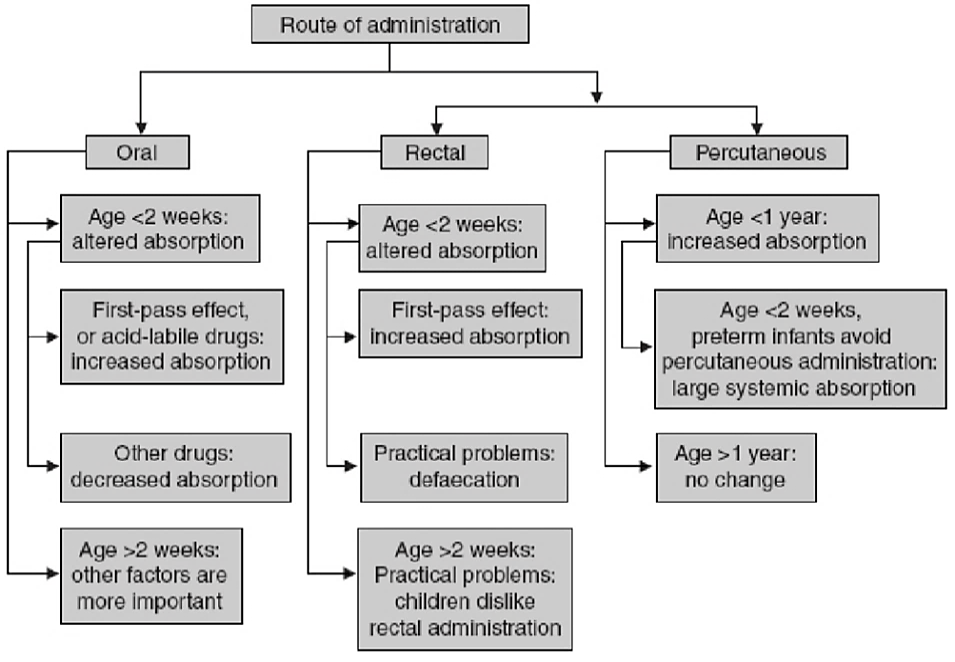
\includegraphics[width=.9\linewidth]{./pediatrie_administration.png}
\end{center}
\section{Posologies}
\label{sec:org34acef9}
\begin{itemize}
\item Posologie de l'enfant:
\[
  P_{enfant} = \frac{ S_{corporelle} \times D_{adulte} }{1.75}
  \]
\item Modifier selon les résultats biologiques:
\begin{itemize}
\item Fonctions rénales
\item Ionogramme sanguin
\end{itemize}
\item Par rapport aux indications:
\end{itemize}
\section{Erreurs d'Administration}
\label{sec:org2697cdb}
\begin{itemize}
\item IV: 48\% \emph{Facteur 10-100}
\item Formes buvables: Confusion \uline{mg/mL} et \uline{mg/kg}
\item Forme galénique non adaptée
\item Application cutanée: \textbf{passage systémique}
\end{itemize}
\section{Effets Indésirables}
\label{sec:org8b16733}
\subsection{Croissance}
\label{sec:orgb55ff2b}
\begin{itemize}
\item Fluoroquinolones: contre-indiquées si < 8 ans \emph{sauf mucoviscidose}
\item Corticoïdes: ralentissement de la croissance
\item Tétracyclines: dischromie et hypoplasie dentaire
\end{itemize}
\subsection{Reye Syndrome}
\label{sec:orge161649}
\begin{itemize}
\item Associé à l'Aspirine si < 16 ans
\item Description: Atteinte cérébrale non-inflammatoire et hépatique
\end{itemize}
\subsection{Précautions et Contre-indications}
\label{sec:orgf63208c}
\begin{itemize}
\item Acide benzoïque CI < 2 ans:
Risque d'ictère car fortement lié aux PP\footnote{Protéines plasmatiques}
\item Camphre: CI < 30 mois
Risque de convulsions
\item Acide borique et borate de Sodium \emph{(Talc, Cold Crean)}: CI < 3 ans
Risque de convulsions
\end{itemize}
\section{Formes Pharmaceutiques: Mésusage}
\label{sec:org929dc2e}
\begin{center}
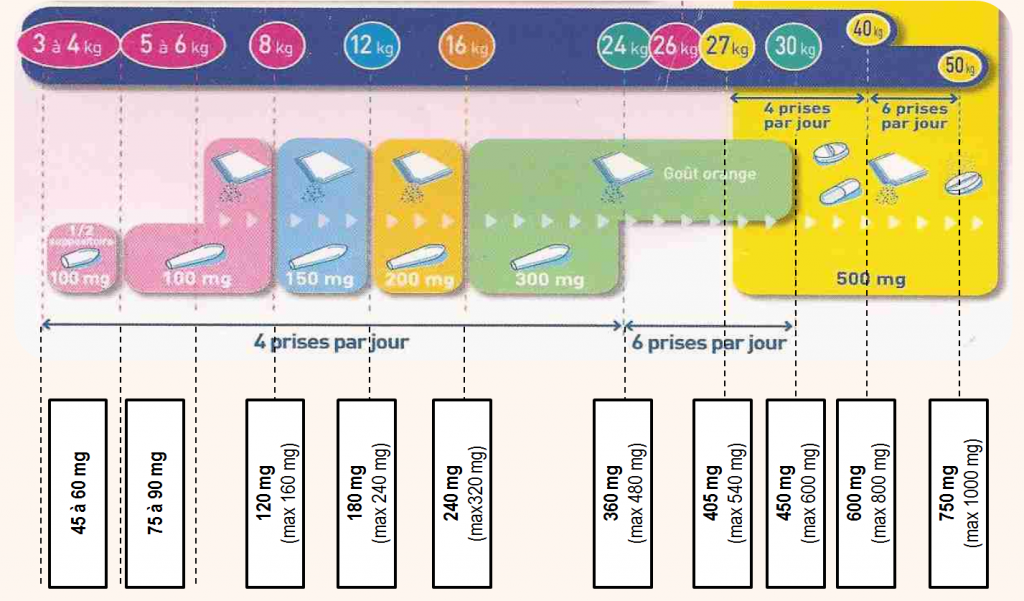
\includegraphics[width=.9\linewidth]{./pedia_galenique.png}
\end{center}
\subsection{Formes Orales Liquides}
\label{sec:orgc4b68d7}
\begin{itemize}
\item Flacon multidose
\item Utilisation de présentation adulte
\item Instrument de mesure non adapté
\item Conservation
\item Absence de date d'ouverture
\item Prescription en unité différente de l'unité indiquée
\end{itemize}
\subsection{Formes Sèches}
\label{sec:orgc1dce10}
\begin{itemize}
\item Prescription de demi ou quart de comprimé
\item Forme galénique inadaptée à l'âge
\item Déconditionnement de médicament
\begin{itemize}
\item Ouverture des gélules
\item Dispersion dans nourriture semi-solide
\item Dissolution dans un liquide
\item Broyage des comprimés
\item Fractionnement
\end{itemize}
\end{itemize}
\end{document}